\begin{figure}[t]
\begin{center}
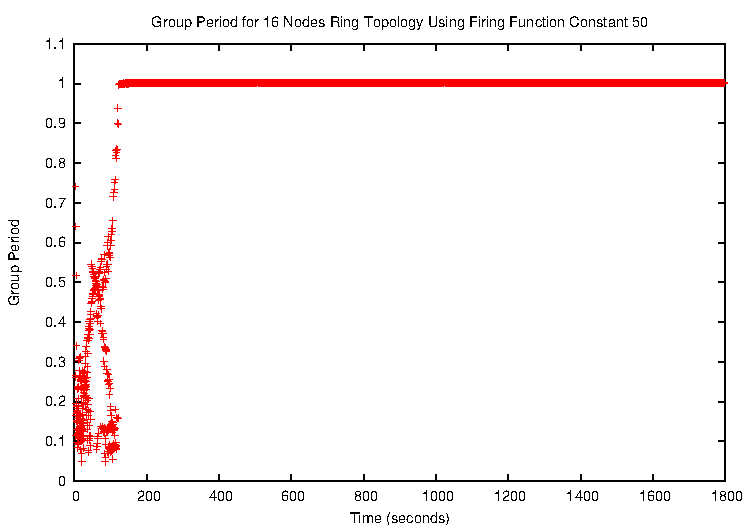
\includegraphics[width=1.0\hsize]{./figures/5-Jan-2005-1-RING-NODES-16-50CONSTANT-GROUP-PERIOD.pdf}
\end{center}
\caption{{\small {\bf Group period for 16 node ring topology with firing function constant 50.}}} 
%{\em This figure shows...}}}
\label{fig:rgp}
\end{figure}

\begin{figure}[t]
\begin{center}
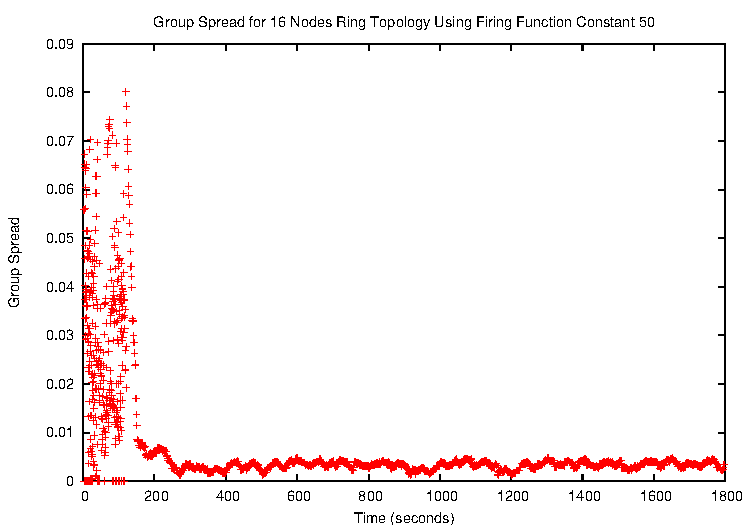
\includegraphics[width=1.0\hsize]{./figures/5-Jan-2005-1-RING-NODES-16-50CONSTANT-GROUP-SPREAD.pdf}
\end{center}
\caption{{\small {\bf Group spread for 16 node ring topology with firing function constant 50.}}}
%{\em This figure shows...}}}
\label{fig:rgs}
\end{figure}

\begin{figure}[t]
\begin{center}
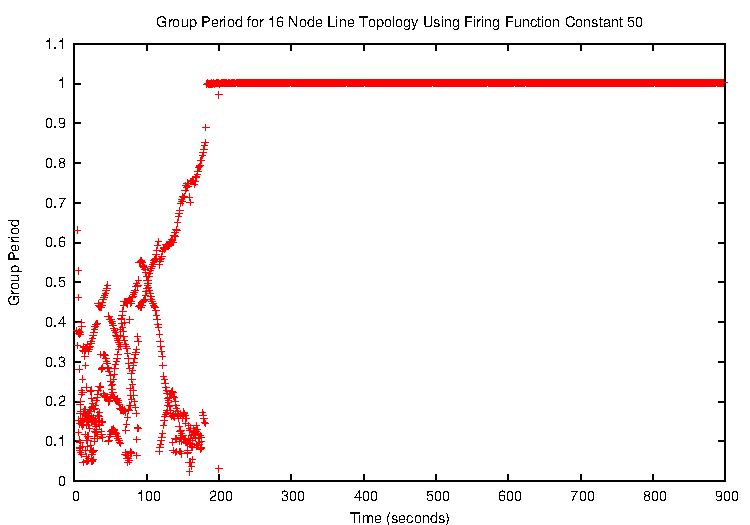
\includegraphics[width=1.0\hsize]{./figures/5-Jan-2005-1-LINE-NODES-16-50CONSTANT-GROUP-PERIOD.pdf}
\end{center}
\caption{{\small {\bf Group period for 16 node line topology with firing function constant 50.} }}
%{\em This figure shows...}}}
\label{fig:lgp}
\end{figure}

\begin{figure}[t]
\begin{center}
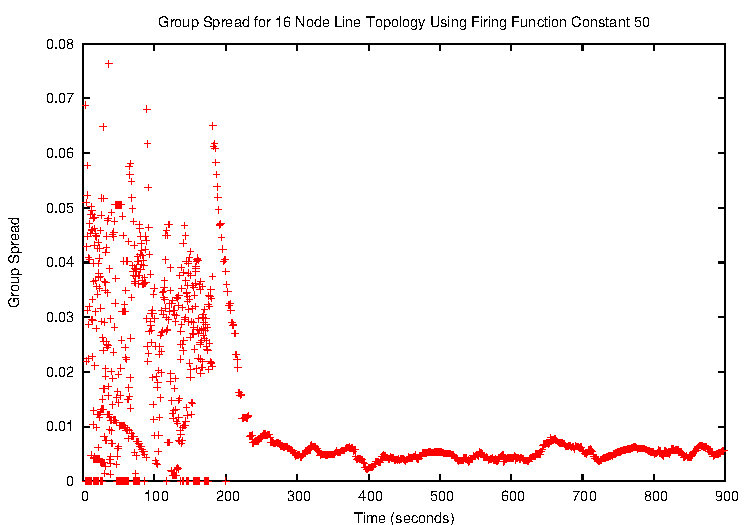
\includegraphics[width=1.0\hsize]{./figures/5-Jan-2005-1-LINE-NODES-16-50CONSTANT-GROUP-SPREAD.pdf}
\end{center}
\caption{{\small {\bf Group spread for 16 node line topology with firing function constant 50.} }}
%{\em This figure shows...}}}
\label{fig:lgs}
\end{figure}

\begin{figure}[t]
\begin{center}
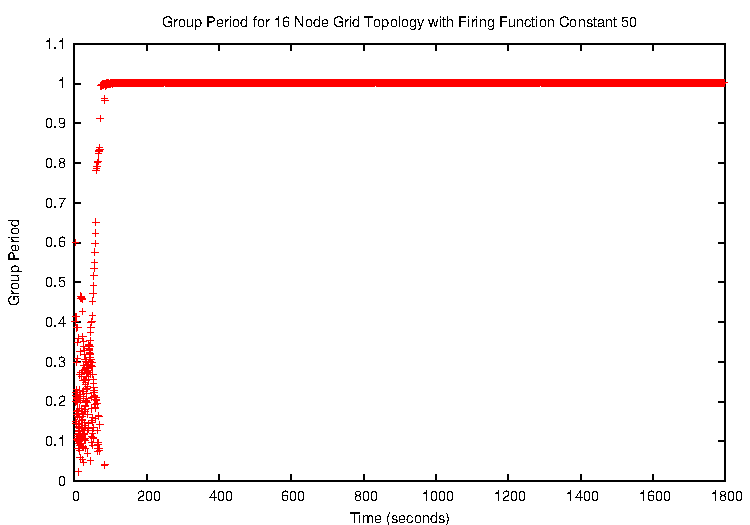
\includegraphics[width=1.0\hsize]{./figures/5-Jan-2005-1-GRID-NODES-16-50CONSTANT-GROUP-PERIOD.pdf}
\end{center}
\caption{{\small {\bf Group period for 16 node 4by4 regular grid topology with firing function constant 50.} }}
%{\em This figure shows...}}}
\label{fig:ggp}
\end{figure}


\begin{figure}[t]
\begin{center}
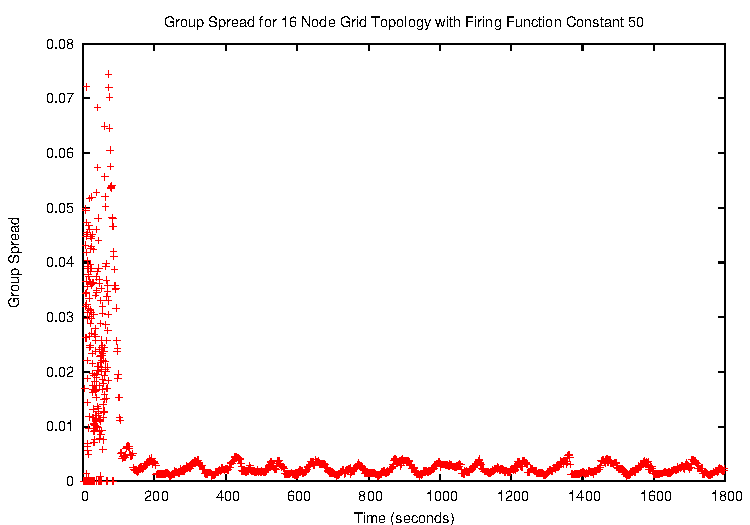
\includegraphics[width=1.0\hsize]{./figures/5-Jan-2005-1-GRID-NODES-16-50CONSTANT-GROUP-SPREAD.pdf}
\end{center}
\caption{{\small {\bf Group spread for 16 node 4by4 regular grid topology with firing function constant 50.} }}
%{\em This figure shows...}}}
\label{fig:ggs}
\end{figure}


\begin{figure}[t]
\begin{center}
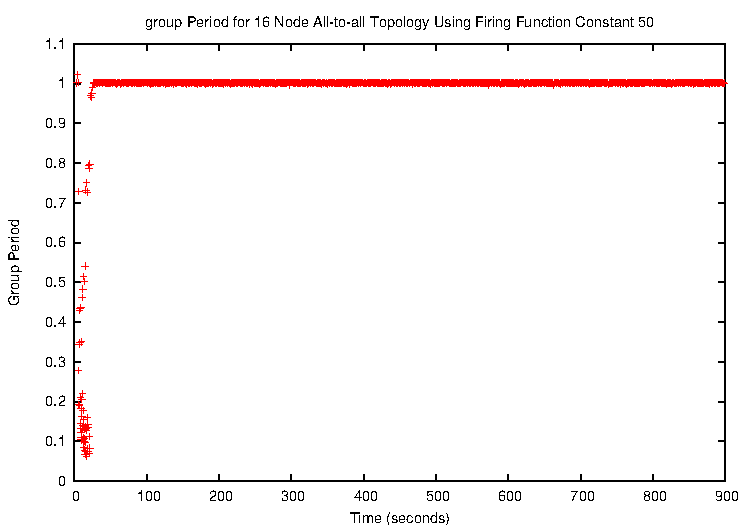
\includegraphics[width=1.0\hsize]{./figures/5-Jan-2005-1-ALL-NODES-16-50CONSTANT-GROUP-PERIOD.pdf}
\end{center}
\caption{{\small {\bf Group period for 16 node all-to-all topology with firing function constant 50.} }}
%{\em This figure shows...}}}
\label{fig:agp}
\end{figure}

\begin{figure}[t]
\begin{center}
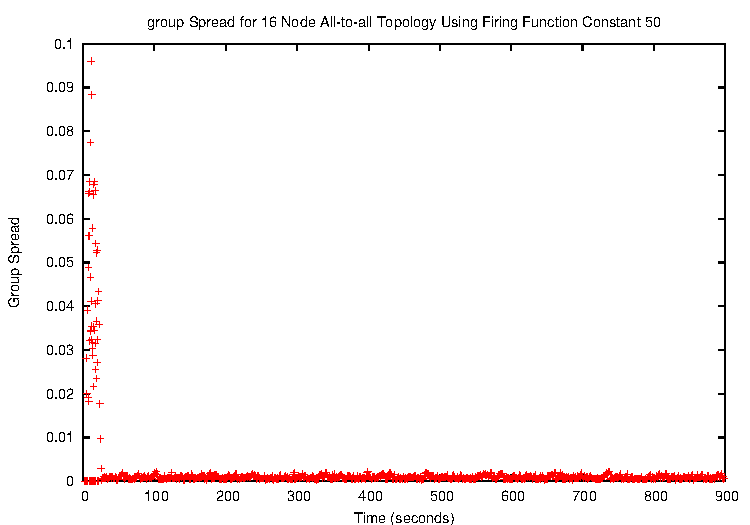
\includegraphics[width=1.0\hsize]{./figures/5-Jan-2005-1-ALL-NODES-16-50CONSTANT-GROUP-SPREAD.pdf}
\end{center}
\caption{{\small {\bf Group spread for 16 node all-to-all topology with firing function constant 50.} }}
%{\em This figure shows...}}}
\label{fig:ags}
\end{figure}


